\section{SgxMonitor: Model Examples}
\label{sec:model-examples_sgxmonitor}

In this section, we discuss the application of SgxMonitor model 
(Section~\ref{sec:model_sgxmonitor}) over two important Intel SGX SDK 
mechanisms:
the outside function interaction (Section~\ref{ssec:ocall-example}) and the 
exception handling (Section~\ref{ssec:exception-handling}).

\paragraph{Transaction syntax.}
For the sake of simplicity, we indicate the transactions in 
tables~\ref{tbl:transactions} and~\ref{tbl:transactions-exception} with the 
following syntax:
$$
T = P \cup [s].
$$
$T$ is composed by any \emph{valid} sequence of \emph{generic actions} $P$ 
(according to the specification of Section~\ref{sec:model_sgxmonitor}) that 
terminates with the \emph{stop action} $s$.
In case $T$ does not contain any \emph{generic action}, we omit $P$.

\subsection{Outside Function Modeling}
\label{ssec:ocall-example}

Figure~\ref{fig:outside-function} shows the application of SgxMonitor to the 
enclave \emph{outside function} interaction.

After the enclave initialization, the host invokes a \emph{secure 
function}, which activates an \texttt{EENTER} opcode with the 
\texttt{idx} greater or equal than \emph{zero} (\ie $T^\text{ECALL}$).
From this point, the \emph{secure function} can evolve in two ways:
\begin{enumerate*}[label=(E\arabic*)]
	\item it does not need any interaction with the host, thus it performs an 
	ERET; or 
	\item it requires an interaction with the host, thus it performs an ORET.
\end{enumerate*}
In case (E1), the enclave does not generate any context and, therefore,
it performs a valid execution path that ends with an 
\texttt{EEXIT} opcode (\ie $T^{\text{ERET}}$).
In case (E2), instead, we need two steps to accomplish an OCALL:
\begin{enumerate*}[label=(\roman*)]
	\item generating an \texttt{ocall\_context} (\ie $T^\text{OCALL1}$), and
	\item invoking the \emph{outside function} (\ie $T^\text{OCALL2}$).
\end{enumerate*}

Once the \emph{outside function} needs to resume the \emph{secure function} 
execution, it invokes an ORET, that is composed by two steps: 
\begin{enumerate*}[label=(\roman*)]
	\item the execution enters in the enclave (\ie $T^\text{ORET1}$), and
	\item the \texttt{ocall\_context} is restored (\ie $T^\text{ORET2}$).
\end{enumerate*}
From this point ahead, the \emph{secure function} can exit the enclave
through an ERET (E1) or perform further OCALLs (E2).

\begin{figure}[t]
	\centering
	\begin{subfigure}[b]{0.43\textwidth}
		\centering
		\begin{tabular}{ll}
			\toprule 
			\textbf{Transaction} & \textbf{Definition} \\ \midrule
			$T^\text{ECALL}$ & $[(\text{N}, \texttt{src}, 
			\texttt{idx})_{\texttt{idx} \geq 0}]$ \\ 
			$T^\text{ERET}$ & $P \cup [(\text{T},\texttt{src},\oslash)]$ \\
			$T^\text{OCALL1}$ & $P \cup [(\text{G}, \texttt{src}, 
			\texttt{ctx})]$ \\ 
			$T^\text{OCALL2}$ & $P \cup [(\text{D},\texttt{src},\oslash)]$ 
			\\ 
			$T^\text{ORET1}$ & $[(\text{N}, \texttt{src}, 
			\texttt{idx})_{\texttt{idx} = -2}]$ \\
			$T^\text{ORET2}$ & $P \cup [(\text{C}, \texttt{src}, 
			\texttt{ctx})]$ \\
			\bottomrule
		\end{tabular} 
		\caption{Transaction definition of SgxMonitor model for the 
		\emph{outside function} interaction.}
		\label{tbl:transactions}
    \end{subfigure}
	\hfill
	\begin{subfigure}[b]{0.56\textwidth}
		\centering
		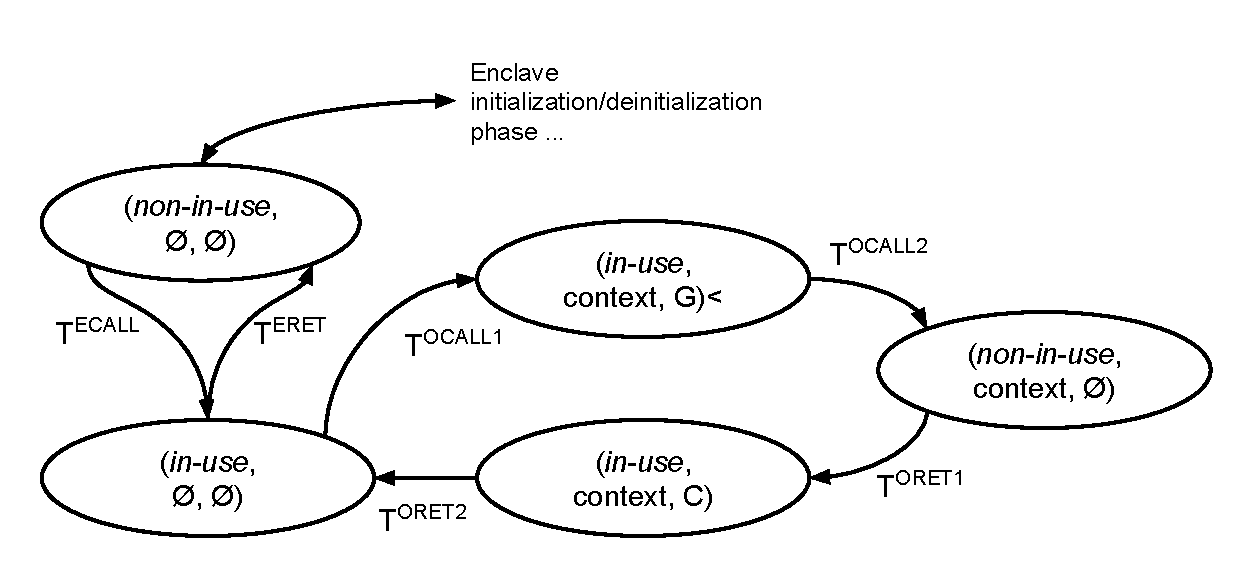
\includegraphics[width=\linewidth]{fig_c6/my-model.pdf}
		\caption{SgxMonitor representation of \emph{outside functions} 
		interaction.}
		\label{fig:my-model}
	\end{subfigure}
	\caption[SGX \emph{outside functions} interaction modeling.]{Example of 
	\emph{outside functions} interaction modeling.
	We show the FSM representation and the transaction definitions, 
	respectively.}
	\label{fig:outside-function}
\end{figure}
\begin{figure}[t]
\centering
\begin{subfigure}[b]{0.43\textwidth}
	\centering
	\begin{tabular}{ll}
		\toprule 
		\textbf{Transaction} & \textbf{Definition} \\ \midrule		
		\texttt{AEX} & \emph{handled at microcode level} \\
		$T^\text{THD1}$ & $[(\text{N}, \texttt{src}, 
		\texttt{idx})_{\texttt{idx} = -3}]$ \\
		$T^\text{THD2}$ & $P \cup [(\text{J}, \texttt{src}, \texttt{ctx})]$ \\
		$T^\text{THD3}$ & $P \cup [(\text{T}, \texttt{src}, \oslash)]$ \\
		$T^\text{ERESUME}$ & $P \cup [(\text{R}, \texttt{src}, \oslash)]$ \\
		$T^\text{IHD1}$ & $P \cup [(\text{K}, \texttt{src}, \texttt{ctx})]$ \\
		$T^\text{IHD2}$ & $P \cup [(\text{J}, \texttt{src}, \texttt{ctx})]$ \\
		$T^\text{CONT}$ & $P \cup [(\text{K}, \texttt{src}, \texttt{ctx})]$ 
		\\		
		\bottomrule
	\end{tabular} 
	\caption{Transaction definition of SgxMonitor model for the exception 
		handling interaction.}
	\label{tbl:transactions-exception}
\end{subfigure}
\hfill
\begin{subfigure}[b]{0.5\textwidth}
	\centering
	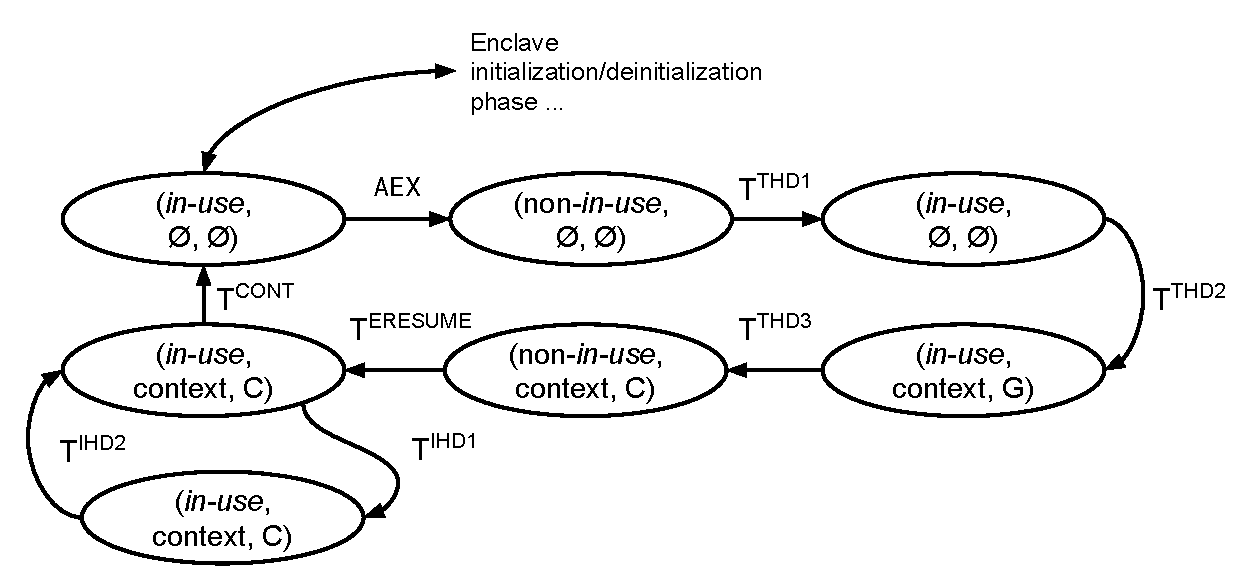
\includegraphics[width=\linewidth]{fig_c6/my-model-exception.pdf}
	\caption{SgxMonitor representation of exception handling.}
	\label{fig:my-model-exception}
\end{subfigure}
\caption[SGX \emph{exception handling} modeling.]{Example of \emph{exception 
handling} modeling. We show the FSM representation and the transaction 
definitions, respectively.}
\label{fig:exception-handling}
\end{figure}

\subsection{Exception Handling Modeling}
\label{ssec:exception-handling}

In Figure~\ref{fig:my-model-exception}, we depict the SgxMonitor 
representation 
of the SGX SDK exception handling.
Overall, the SGX SDK handles exceptions in two phases, called \emph{trusted 
handle} (TH) and \emph{internal handle} (IH), respectively.
In the first phase (TH), the SGX interrupts its 
execution as a result of an \texttt{AEX}, and passes the control to the host.
As soon as an exception is triggered, the microcode saves the CPU
registers in a dedicated page, called SSA, for later 
stages~\cite{costan2016intel}.
After an \texttt{AEX}, the SDK expects the invocation of a dedicated 
\emph{secure function}, called \texttt{trts\_handle\_exception}, which index is 
$-3$ (\ie T$^\text{THD1}$).
This function fills an \texttt{sgx\_exception\_info\_t} structure with the 
values previously stored in the SSA (\ie T$^\text{THD2}$).
At the end of (TH), the enclave is ready for the second phase (IH) and thus it
leaves the control to the host (\ie T$^\text{THD3}$).
The host invokes an \texttt{ERESUME} to activate
the \texttt{internal\_handle\_exception} routine (\ie T$^\text{ERESUME}$).
Now, the enclave iterates among the custom handlers eventually registered
(\ie T$^\text{IHD1}$ and T$^\text{IHD2}$).
Each custom handler attempts at fixing the exception by analyzing the 
\texttt{sgx\_exception\_info\_t}, possibly altering it.
Therefore, we update the enclave internal state at each iteration.
After invoking all the internal handlers, the SGX SDK uses the
\texttt{continue\_execution} routine to resume the \emph{secure function} (\ie 
T$^\text{CONT}$).
Finally, if the exception is properly handled, the \emph{secure function} 
will continue, otherwise, a new \texttt{AEX} happens and the 
exception workflow starts again.

